\documentclass{article}%standalone can be used
\usepackage[utf8]{inputenc}
\usepackage{tikz}
\usetikzlibrary{shapes.geometric, arrows, chains, calc}

\tikzset{
    green/.style  = {draw, rectangle, minimum width=2cm, minimum height=1cm, text centered, text width=1.2cm, font=\footnotesize, draw=black, fill=green!30},
    blue/.style   = {draw, rectangle, minimum width=8cm+3\pgflinewidth, minimum height=1cm, text centered, text width=5.0cm, font=\footnotesize, draw=black, fill=blue!30},
    yellow/.style = {draw, rectangle, minimum width=8cm+3\pgflinewidth, minimum height=1cm, text centered, text width=5.0cm, font=\footnotesize, draw=black, fill=yellow!30},
}

\begin{document}
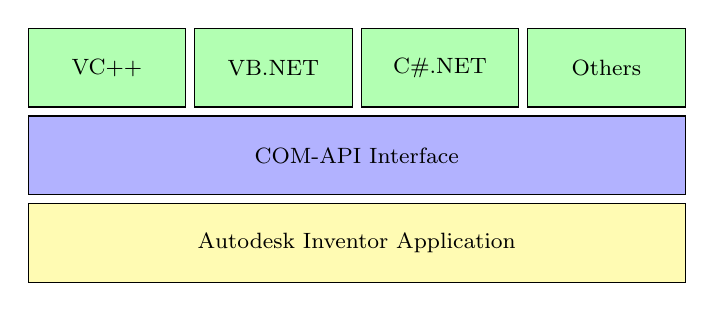
\begin{tikzpicture}[start chain=1 going right, start chain=2 going below, node distance=1mm]
  \node [name=r1c1, on chain=1, green] {VC++};
  \node [name=r1c2, on chain=1, green] {VB.NET};
  \node [name=r1c3, on chain=1, green] {C\#.NET};
  \node [name=r1c4, on chain=1, green] {Others};
  \draw let \p1=($(r1c4.east)-(r1c1.west)$), \n1 = {veclen(\x1,\y1)} in node [name=r2c1, on chain=2, blue, anchor=north west, yshift=-1mm, minimum width=\n1-\pgflinewidth] at (r1c1.south west) {COM-API Interface};
  \draw let \p1=($(r1c4.east)-(r1c1.west)$), \n1 = {veclen(\x1,\y1)} in node [name=r3c1, on chain=2, yellow, minimum width=\n1-\pgflinewidth] {Autodesk Inventor Application};
\end{tikzpicture}
\end{document}
